% Determines the type of document and font size
\documentclass[12pt,a4paper]{article}
% Font control
\usepackage{mathptmx} % Times Roman Font
\usepackage{helvet} % Arial/Helvetica font
\renewcommand{\familydefault}{\sfdefault} % Makes serif text all Helvetica
% Set up the page margins
\usepackage[left=2.5cm, right=2.5cm, top=2.5cm]{geometry}
% Allow graphics
\usepackage{graphicx}
% put graphs in place
\usepackage[section]{placeins}
% caption font
\usepackage[font=small,labelfont=bf]{caption}
% float package: picture position
\usepackage{float}
% symbols
\usepackage{textcomp, gensymb}
% hyperref
\usepackage{hyperref}
% Add your report title here
\title{OCNG/ATMO 651 Final Project: Linear Inverse Model of Tropical Sea Surface Temperatures}
% Add your name here
\author{Jinjun Liu}
\date{\today}

% The start of the document
\begin{document}
% This adds the title page
\maketitle
\thispagestyle{empty}
% This adds the abstract
\begin{abstract}

In this project, we employ the linear inverse model (LIM) to predict sea surface tempratures anomalies (SSTAs).

\end{abstract}

\tableofcontents

% Move to a new page and set the page numbering from here
\clearpage % moves to the next page
\pagenumbering{arabic}

\section{Introduction} % The start of a new section

Penland and Magorian \cite{Penland1993} proposed a linear inverse model (LIM) to predict sea surface tempratures (SSTs) in the region of the equatorial Pacific Ocean. The root mean squared (rms) prediction error at a leading time of 9 month is about half degree celcius. They also found that the LIM can be used to predict the SSTs in the tropical Atlantic Ocean \cite{Penland1996}. In this project, we employ the LIM to predict sea surface tempratures anomalies (SSTAs).
 \cite{Penland1993}. They then use the LIM to predict the tropical Atlantic SST \cite{Penland1996}.

\section{Dataset and Method}\label{dataset-method}

We use the NCEP/NCAR (National Centers for Environmental Prediction/National Center for Atmospheric Research) reanalysis SST as the dataset to build the LIM and make predictions. This dataset used in this project contains monthly-mean SSTs from January 1948 to September 2017. We divide the dataset into two parts: the training dataset and the test dataset. The training dataset contains the SSTs from January 1948 to December 1999, and the test dataset contains the SSTs from January 2000 to September 2017. We use the training dataset to build the LIM and use the test dataset to evaluate the performance of the LIM.

The Python script that processes the data and generates the figures is available at \url{https://github.com/jinjunliu/atmo-651/blob/master/Final/ATMO651\_Final.ipynb}.

\section{Results}\label{results}

\subsection{EOF decomposition of SSTs}\label{eof-decomposition}

\begin{figure}[htbp]
\centering
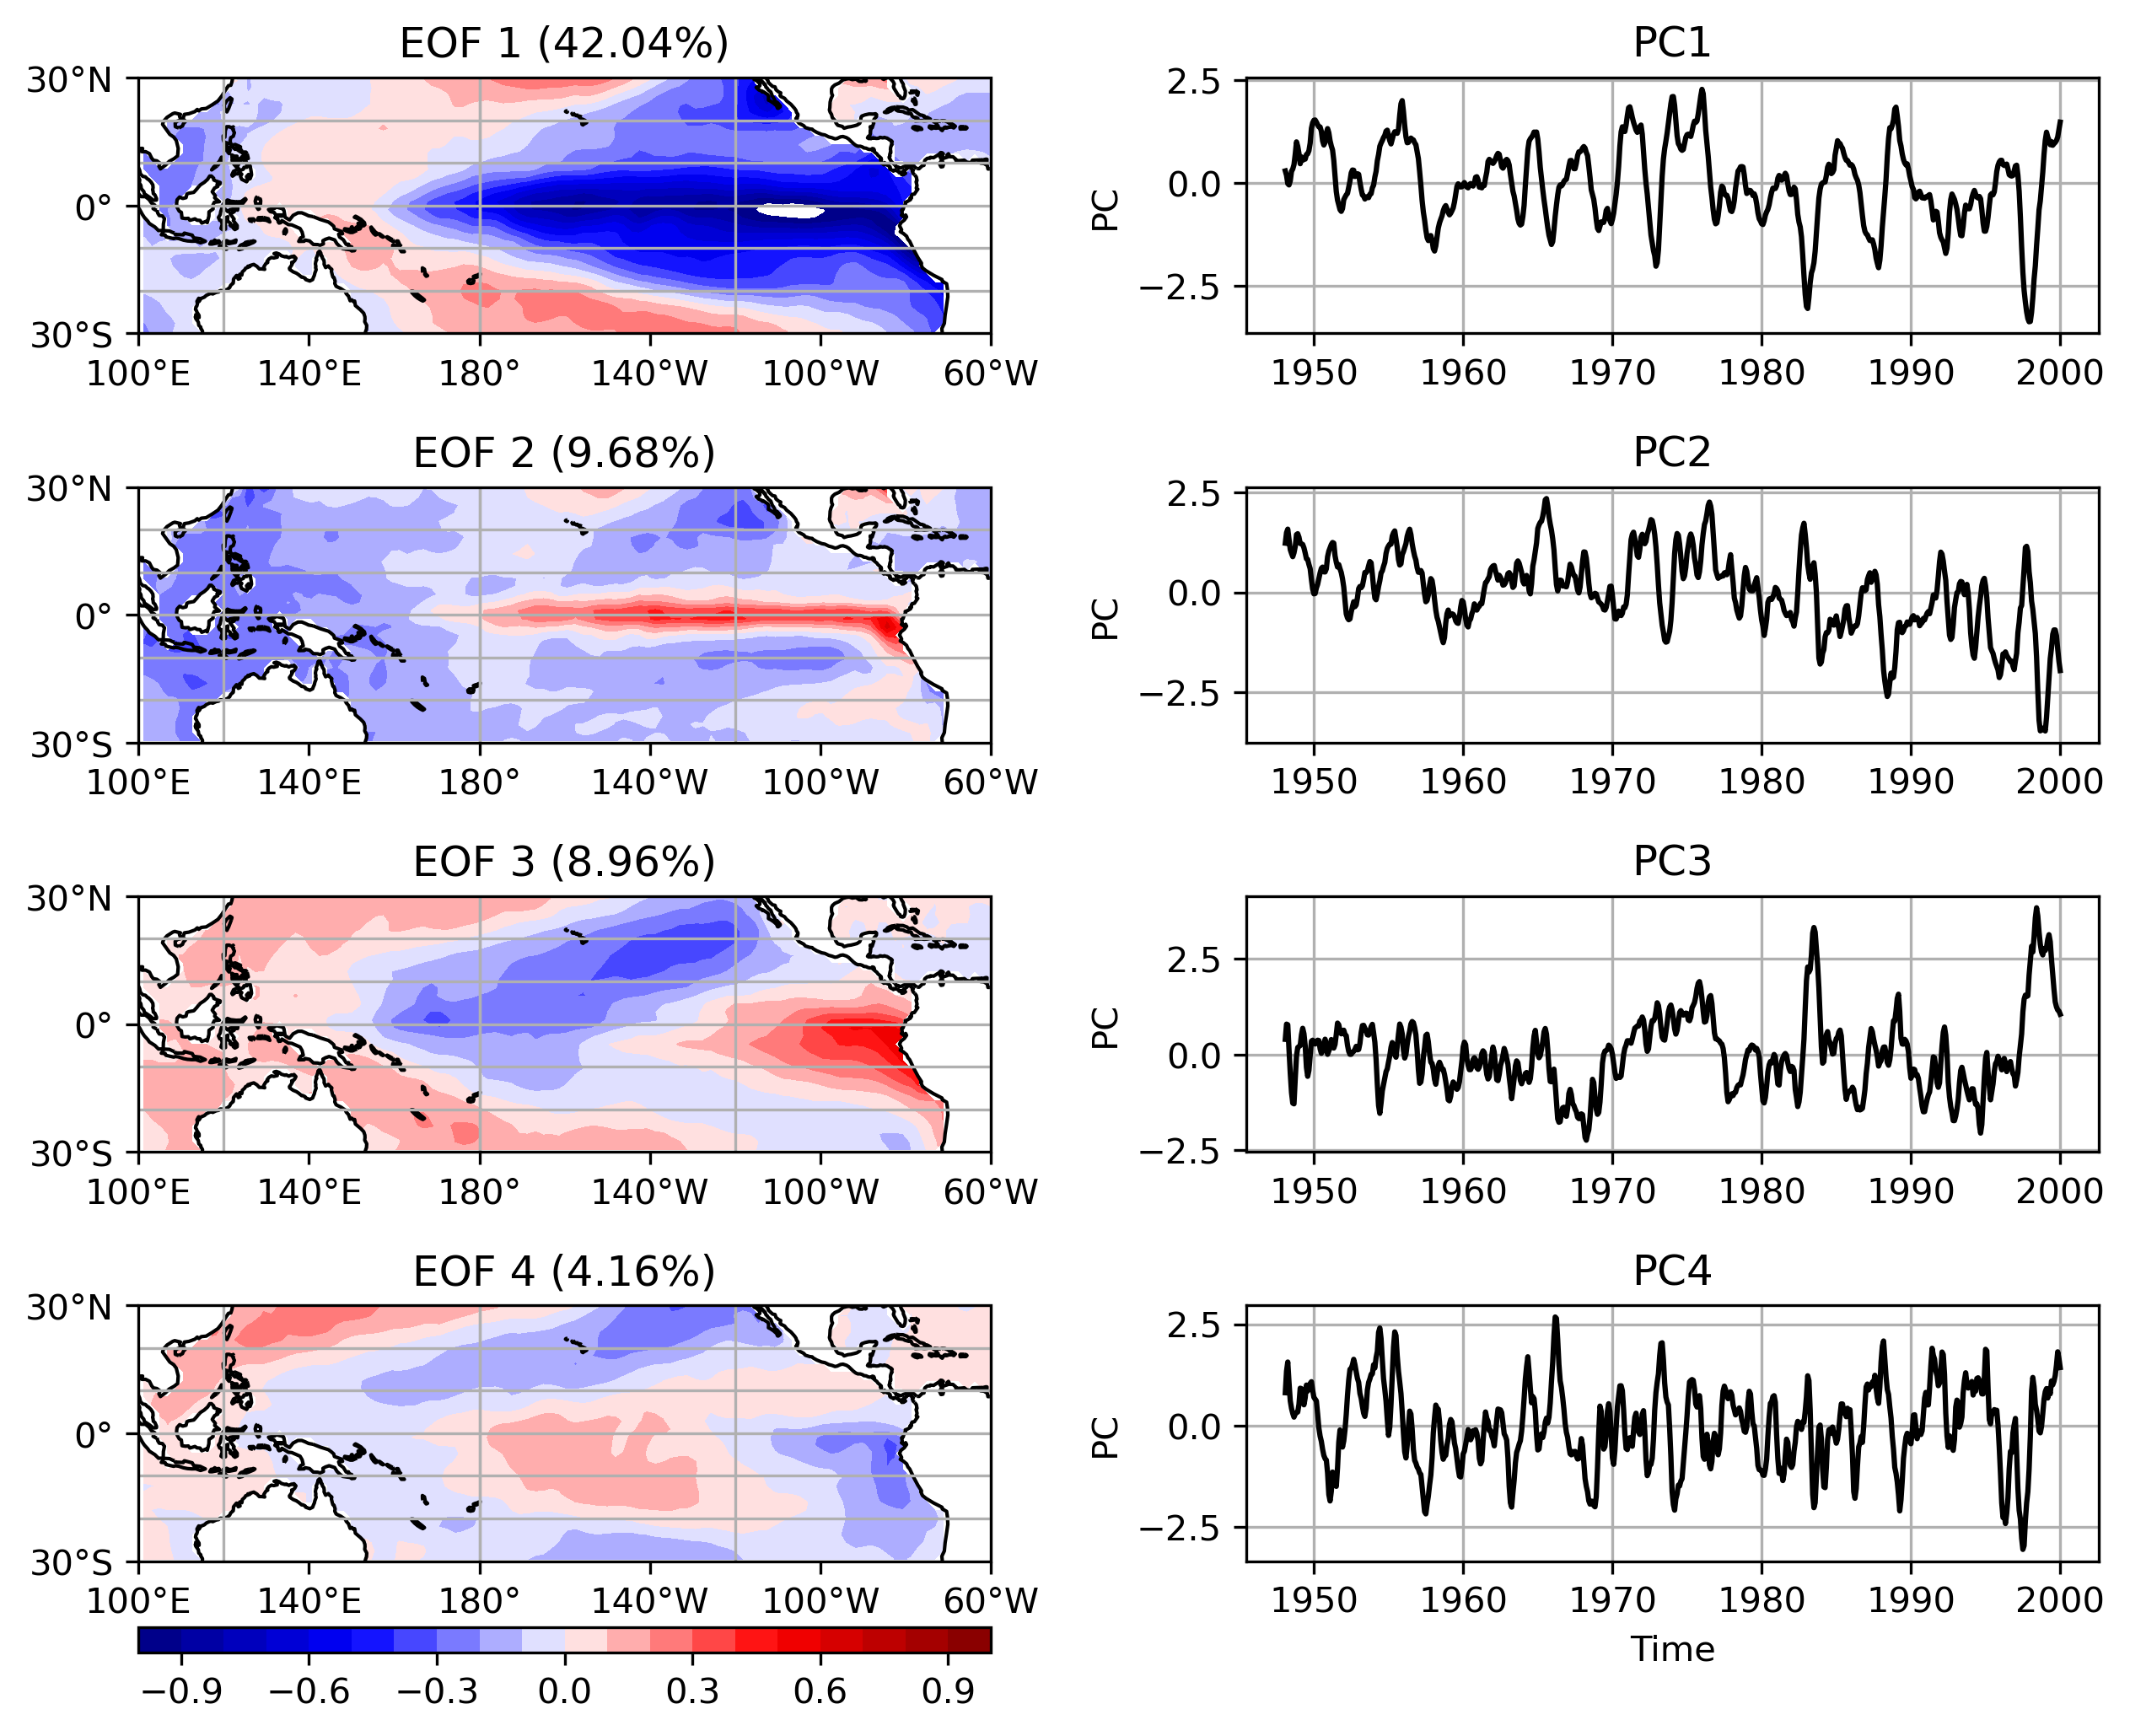
\includegraphics[width=0.8\textwidth]{figures/EOFs_PCs.png}
\caption{EOF decomposition of SSTs.}
\label{fig:EOFs_PCs}
\end{figure}

\subsection{Linear inverse model in EOF space}\label{lim-eof-space}

\section{Aknowledgements}\label{acknowledgements}

Thanks to Dr. Ping Chang for providing the datasets and the guidance.

\bibliographystyle{abbrv}
\bibliography{library}

\end{document}
